% A LaTeX template for EXECUTIVE SUMMARY of the MSc Thesis submissions to 
% Politecnico di Milano (PoliMi) - School of Industrial and Information Engineering
%
% S. Bonetti, A. Gruttadauria, G. Mescolini, A. Zingaro
% e-mail: template-tesi-ingind@polimi.it
%
% Last Revision: October 2021
%
% Copyright 2021 Politecnico di Milano, Italy. NC-BY

\documentclass[11pt,a4paper,twocolumn]{article}

%------------------------------------------------------------------------------
%	REQUIRED PACKAGES AND  CONFIGURATIONS
%------------------------------------------------------------------------------
% PACKAGES FOR TITLES
\usepackage{titlesec}
\usepackage{color}

% PACKAGES FOR LANGUAGE AND FONT
\usepackage[utf8]{inputenc}
\usepackage[english]{babel}
\usepackage[T1]{fontenc} % Font encoding

% PACKAGES FOR IMAGES
\usepackage{graphicx}
\graphicspath{{Images/}} % Path for images' folder
\usepackage{eso-pic} % For the background picture on the title page
\usepackage{subfig} % Numbered and caption subfigures using \subfloat
\usepackage{caption} % Coloured captions
\usepackage{transparent}

% STANDARD MATH PACKAGES
\usepackage{amsmath}
\usepackage{amsthm}
\usepackage{bm}
\usepackage[overload]{empheq}  % For braced-style systems of equations

% PACKAGES FOR TABLES
\usepackage{tabularx}
\usepackage{longtable} % tables that can span several pages
\usepackage{colortbl}

% PACKAGES FOR ALGORITHMS (PSEUDO-CODE)
\usepackage{algorithm}
\usepackage{algorithmic}

% PACKAGES FOR REFERENCES & BIBLIOGRAPHY
\usepackage[colorlinks=true,linkcolor=black,anchorcolor=black,citecolor=black,filecolor=black,menucolor=black,runcolor=black,urlcolor=black]{hyperref} % Adds clickable links at references
\usepackage{cleveref}
% I CHANGED BELOW TWO LINES
\usepackage[numbers,sort&compress]{natbib}
\bibliographystyle{unsrtnat}

% PACKAGES FOR THE APPENDIX
\usepackage{appendix}

% PACKAGES FOR ITEMIZE & ENUMERATES 
\usepackage{enumitem}

% OTHER PACKAGES
\usepackage{amsthm,thmtools,xcolor} % Coloured "Theorem"
\usepackage{comment} % Comment part of code
\usepackage{fancyhdr} % Fancy headers and footers
\usepackage{lipsum} % Insert dummy text
\usepackage{tcolorbox} % Create coloured boxes (e.g. the one for the key-words)
\usepackage{stfloats} % Correct position of the tables

%-------------------------------------------------------------------------
%	NEW COMMANDS DEFINED
%-------------------------------------------------------------------------
% EXAMPLES OF NEW COMMANDS -> here you see how to define new commands
\newcommand{\bea}{\begin{eqnarray}} % Shortcut for equation arrays
\newcommand{\eea}{\end{eqnarray}}
\newcommand{\e}[1]{\times 10^{#1}}  % Powers of 10 notation
\newcommand{\mathbbm}[1]{\text{\usefont{U}{bbm}{m}{n}#1}} % From mathbbm.sty
\newcommand{\pdev}[2]{\frac{\partial#1}{\partial#2}}
% NB: you can also override some existing commands with the keyword \renewcommand

%----------------------------------------------------------------------------
%	ADD YOUR PACKAGES (be careful of package interaction)
%----------------------------------------------------------------------------
\usepackage{pifont}
\newcommand{\cmark}{\ding{51}}%
\newcommand{\xmark}{\ding{55}}%

\usepackage{graphicx}
\newcommand{\Csharp}{%
  {\settoheight{\dimen0}{C}C\kern-.05em \resizebox{!}{\dimen0}{\raisebox{\depth}{\# }}}}
%----------------------------------------------------------------------------
%	ADD YOUR DEFINITIONS AND COMMANDS (be careful of existing commands)
%----------------------------------------------------------------------------


% Do not change Configuration_files/config.tex file unless you really know what you are doing. 
% This file ends the configuration procedures (e.g. customizing commands, definition of new commands)
% Define blue color typical of polimi
\definecolor{bluepoli}{cmyk}{0.4,0.1,0,0.4}

% Custom theorem environments
\declaretheoremstyle[
  headfont=\color{bluepoli}\normalfont\bfseries,
  bodyfont=\color{black}\normalfont\itshape,
]{colored}

% Set-up caption colors
\captionsetup[figure]{labelfont={color=bluepoli}} % Set colour of the captions
\captionsetup[table]{labelfont={color=bluepoli}} % Set colour of the captions
\captionsetup[algorithm]{labelfont={color=bluepoli}} % Set colour of the captions

\theoremstyle{colored}
\newtheorem{theorem}{Theorem}[chapter]
\newtheorem{proposition}{Proposition}[chapter]

% Enhances the features of the standard "table" and "tabular" environments.
\newcommand\T{\rule{0pt}{2.6ex}}
\newcommand\B{\rule[-1.2ex]{0pt}{0pt}}

% Pseudo-code algorithm descriptions.
\newcounter{algsubstate}
\renewcommand{\thealgsubstate}{\alph{algsubstate}}
\newenvironment{algsubstates}
  {\setcounter{algsubstate}{0}%
   \renewcommand{\STATE}{%
     \stepcounter{algsubstate}%
     \Statex {\small\thealgsubstate:}\space}}
  {}

% New font size
\newcommand\numfontsize{\@setfontsize\Huge{200}{60}}

% Title format: chapter
\titleformat{\chapter}[hang]{
\fontsize{50}{20}\selectfont\bfseries\filright}{\textcolor{bluepoli} \thechapter\hsp\hspace{2mm}\textcolor{bluepoli}{|   }\hsp}{0pt}{\huge\bfseries \textcolor{bluepoli}
}

% Title format: section
\titleformat{\section}
{\color{bluepoli}\normalfont\Large\bfseries}
{\color{bluepoli}\thesection.}{1em}{}

% Title format: subsection
\titleformat{\subsection}
{\color{bluepoli}\normalfont\large\bfseries}
{\color{bluepoli}\thesubsection.}{1em}{}

% Title format: subsubsection
\titleformat{\subsubsection}
{\color{bluepoli}\normalfont\large\bfseries}
{\color{bluepoli}\thesubsubsection.}{1em}{}

% Shortening for setting no horizontal-spacing
\newcommand{\hsp}{\hspace{0pt}}

\makeatletter
% Renewcommand: cleardoublepage including the background pic
\renewcommand*\cleardoublepage{%
  \clearpage\if@twoside\ifodd\c@page\else
  \null
  \AddToShipoutPicture*{\BackgroundPic}
  \thispagestyle{empty}%
  \newpage
  \if@twocolumn\hbox{}\newpage\fi\fi\fi}
\makeatother

%For correctly numbering algorithms
\numberwithin{algorithm}{chapter}

% Insert here the info that will be displayed into your Title page 
% -> title of your work
\renewcommand{\title}{Design Patterns and Anti-Patterns in Microservices Architecture: A Classification Proposal and Study on Open Source Projects}
% -> author name and surname
\renewcommand{\author}{Ömer Esas}
% -> MSc course
\newcommand{\course}{Computer Science and Engineering - Ingegneria Informatica}
% -> advisor name and surname
\newcommand{\advisor}{Prof. Elisabetta Di Nitto}
% IF AND ONLY IF you need to modify the co-supervisors you also have to modify the file Configuration_files/title_page.tex (ONLY where it is marked)
% \newcommand{\firstcoadvisor}{Name Surname} % insert if any otherwise comment
%\newcommand{\secondcoadvisor}{Name Surname} % insert if any otherwise comment
% -> academic year
\newcommand{\YEAR}{2021-2022}

%-------------------------------------------------------------------------
%	BEGIN OF YOUR DOCUMENT
%-------------------------------------------------------------------------
\begin{document}

%-----------------------------------------------------------------------------
% TITLE PAGE
%-----------------------------------------------------------------------------
% Do not change Configuration_files/TitlePage.tex (Modify it IF AND ONLY IF you need to add or delete the Co-advisors)
% This file creates the Title Page of the document
% DO NOT REMOVE SPACES BETWEEN LINES!

\twocolumn[{\begin{@twocolumnfalse}

\AddToShipoutPicture*{\BackgroundPic}

\hspace{-0.6cm}
\includegraphics[width=0.6\textwidth]{logo_polimi_ing_indinf.eps}

\vspace{-1mm}
\fontsize{0.3cm}{0.5cm}\selectfont \bfseries \textsc{\color{bluePoli} Executive Summary of the Thesis}\\

\vspace{-0.2cm}
\Large{\textbf{\color{bluePoli}{\title}}}\\

\vspace{-0.2cm}
\fontsize{0.3cm}{0.5cm}\selectfont \bfseries \textsc{\color{bluePoli} Laurea Magistrale in \course}\\

\vspace{-0.2cm}
\fontsize{0.3cm}{0.5cm} \selectfont \bfseries Author: \textsc{\textbf{\author}}\\

\vspace{-0.4cm}
\fontsize{0.3cm}{0.5cm}\selectfont \bfseries Advisor: \textsc{\textbf{\advisor}}\\

% if only ONE co-advisor is present:
%\vspace{-0.4cm}
%\fontsize{0.3cm}{0.5cm}\selectfont \bfseries Co-advisor: %\textsc{\textbf{\firstcoadvisor}}\\
% if more than one co-advisors are present:
%\vspace{-0.4cm}
%\fontsize{0.3cm}{0.5cm}\selectfont \bfseries Co-advisors: \textsc{\textbf{\firstcoadvisor}}\textsc{\textbf{\secondcoadvisor}}\\

\vspace{-0.4cm}
\fontsize{0.3cm}{0.5cm}\selectfont \bfseries Academic year: \textsc{\textbf{\YEAR}}

\small \normalfont

\vspace{11pt}

\centerline{\rule{1.0\textwidth}{0.4pt}}

\vspace{15pt}
\end{@twocolumnfalse}}]

\thispagestyle{plain} % In order to not show the header in the first page

%%%%%%%%%%%%%%%%%%%%%%%%%%%%%%
%%     THESIS MAIN TEXT     %%
%%%%%%%%%%%%%%%%%%%%%%%%%%%%%%

%-----------------------------------------------------------------------------
% INTRODUCTION
%-----------------------------------------------------------------------------
\section{Introduction}
\label{sec:introduction}

As tech giants such as Amazon, Netflix and Uber adopted microservices architecture successfully in the past decade, there has been an increase in the microservices research in the academia and greater interest from many companies towards this method of building distributed, fault-tolerant and complex applications.
More research and practical experience led to the emergence of several desirable and undesirable ways of solving problems faced in microservice-based systems, called microservices design patterns and anti-patterns.
In this study, we aim to explore these patterns and anti-patterns, specifically, in terms of classification in the literature and detection of them on a group of open source microservices projects.
We aim to observe the way the patterns and anti-patterns are classified in the literature, check if there exists a common way of classification and propose our own taxonomy in case there is no consensus in the literature.
Then, we select ten open source microservice projects and manually inspect source code to detect the design patterns and anti-patterns of microservices architecture, in order to observe the correlation between the "theory" in the literature and practical cases to some extent.
\\
To the best of our knowledge, there are two studies in the literature that are similar to our work.
The researchers of the first similar study\cite{8719492} inspect a set of thirty open source microservice projects using automated tools that check the dependency files and verify the use of the pattern by checking the documentation of the utilized framework.
The researchers of the second similar study\cite{10.1145/3424771.3424812} manually check sixty seven projects to detect anti-patterns, which they discover as a result of their systematic literature review for microservices anti-patterns.
Our study differs from the two studies in considering not only design patterns or anti-patterns, but both of these good and bad practices, in addition to using only manual inspection on projects that use many different technologies.

%-----------------------------------------------------------------------------
% STATE OF THE ART
%-----------------------------------------------------------------------------

\section{State of the Art}
\label{sec:State of the Art}

To be able to explain the methodology and the results of this study, we see it fit to describe microservices architecture and list its design patterns and anti-patterns, which are obtained from Microsoft Cloud patterns website\cite{microsoft_docs}, microservice patterns book\cite{richardson_book} and two studies about microservices anti-patterns\cite{10.1145/3424771.3424812}\cite{9522227}.
Although we present only the names of design patterns and anti-patterns here to keep it concise, they are explained in detail in the main thesis paper.

\subsection{Microservices Architecture}
\label{subsec:microservice}

In essence, microservice-based applications consists of a number of small software services, that are designed to carry out one business capability of the application.
The system is not divided into technical layers, instead, the whole application domain is partitioned into bounded contexts, each of which is then, ideally, assigned to one small self-sufficient team to implement as a microservice.
The team is responsible for the implementation, deployment and maintenance of the particular microservice, meaning that, they are free to choose their programming language, libraries and frameworks to implement, and free in their choice of CI/CD tools to utilize during various stages of software development.
If required for the particular business capability, the team can persist the data, which is modeled around that bounded context, by making use of a database, again, selected by the team according to the needs and suitability of that particular microservice.
Last but not least, the microservices communicate with each other by means of network calls, using well-defined APIs, and simple protocols like REST over HTTP.
Unlike Service Oriented Architecture (SOA) that utilize Enterprise Service Buses (ESB) with additional capabilities, microservices opt for simple communication infrastructure that can do basic routing of messages, as summarised in the motto "simple endpoints, dumb pipes".
Figure~\ref{fig:monovsmicro} illustrates the microservices architecture characteristics by comparing it with a typical monolithic architecture.

\begin{figure}[H]
\centering
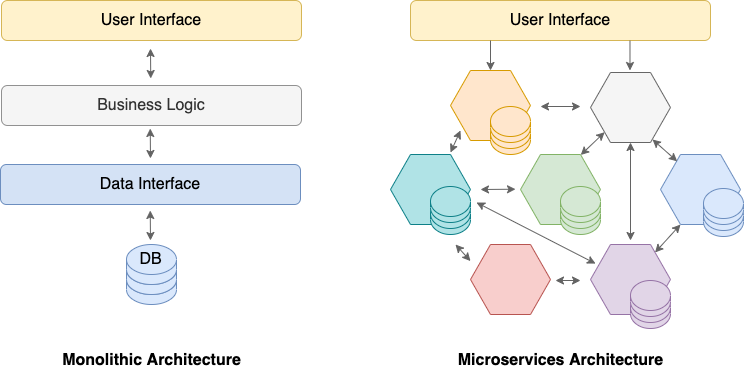
\includegraphics[width=0.40\textwidth]{monovsmicro.png}
\caption{Monolithic vs Microservices Architecture}
\label{fig:monovsmicro}
\end{figure}

\subsection{Design Patterns}
\label{subsec:patterns}

The design patterns of microservices architecture considered in this study are listed below:

\begin{itemize}
    \item API Gateway
    \item Service Mesh with Sidecar
    \item Service Registry and Discovery
    \item Backends for Frontends
    \item Asynchronous Messaging
    \item Database per Service
    \item Saga
    \item API Composition
    \item Command Query Responsibility Segregation (CQRS)
    \item Event Sourcing
    \item Service Instance per Virtual Machine
    \item Service Instance per Container
    \item Serverless
    \item Health Check API
    \item Log Aggregator
    \item Distributed Tracing
    \item Circuit Breaker
\end{itemize}

\subsection{Anti-Patterns}
\label{subsec:anti-patterns}

Similarly, we present the list of anti-patterns considered during this study:

\begin{itemize}
    \item Wrong Cut
    \item Nano Microservice
    \item Mega Microservice
    \item ESB Usage
    \item Hardcoded Endpoints
    \item No API Gateway
    \item Shared Persistence
    \item Shared Libraries
    \item No CI/CD Tools
    \item Multiple Services per Host
    \item No API Versioning
    \item No Health Check
    \item Local Logging
\end{itemize}

\section{Research Methodology}
\label{sec:research_method}

As the goal of this study, we aimed to observe the classification regarding microservices design patterns and anti-patterns in the literature, present one in case there is no consensus, and check the presence of these patterns and anti-patterns in popular open source projects.
Specifically, we established two research questions:
\begin{itemize}
    \item \textbf{RQ1}: Is there a consistent categorization or classification of design patterns and anti-patterns of microservices architecture in the academia?
    If not, what could be an alternative way to classify these design patterns and anti-patterns?
    
    \item \textbf{RQ2}: Which of these design patterns and anti-patterns exist in popular open source microservices applications?
\end{itemize}

To answer first research question, the following steps have been adopted.

\begin{itemize}
    \item In order to find out whether there exists a consistent classification of microservice design patterns and anti-patterns, a literature review on digital libraries such as IEEE Explore, ACM Digital Library, Springer, Scopus, and Google Scholar has been carried out.
    The keywords used in the search queries included "microservice pattern", "microservice pattern classification", "microservice anti-pattern" and "microservice anti-pattern classification".

    \item After initial review of the studies found, few more studies have been added through snowballing technique, and from this extended set, the studies that do not contain a classification or grouping of patterns and anti-patterns have been eliminated.
    
    \item To be able to propose a classification of patterns and anti-patterns on a sound basis, various perspectives through which microservices architecture can be examined needed to be identified.
    For this reason, the systematic mapping studies found in the literature review process have been consulted.
    
    \item Considering the classifications found in the literature and the findings resulted from papers that conducted systematic mapping studies, a classification proposal has been developed.
\end{itemize}

As for the second research question, the following steps have been carried out.

\begin{itemize}
    \item Open source repository hosting service GitHub is queried with he keyword pattern "microservice OR micro-service". 
    To find the most popular projects, the search result is sorted using "most stars" option.

    \item Ten microservice repositories that have the most number of stars are selected.
    While doing so, the repositories that contain libraries, frameworks or tool-kits have been eliminated, in addition to the ones that contain "microservice" keyword but rather implemented using other architectures.
    
    \item Because of the technological heterogeneity among the set of projects, two design patterns, namely "saga" and "shared libraries" which require a competent understanding of the programming language being used and a thorough comprehension of the business logic are excluded from the list of patterns and anti-patterns to be identified.
    
    \item For the detection of the rest of the microservices design patterns and anti-patterns, we manually inspected the repositories and the source codes of projects, without utilizing any automated tool.
    We tried to find any information on the repository page that indicates the use of a particular pattern or anti-pattern, checked the source code and tried to verify the use of a pattern by consulting to the reference document of a library or framework at hand.
    To detect hardcoded IP addresses, we made use of the simple regular expression "\textbackslash b\textbackslash d\{1,3\}\textbackslash .\textbackslash d\{1,3\}\textbackslash .\textbackslash d\{1,3\}\textbackslash .\textbackslash d\{1,3\}\textbackslash b" and examined the context of the found hardcoded IP addresses.
    For patterns and anti-patterns that can be implemented to various extents, such as API composition and shared persistence, we stated the criteria that we used to indicate the presence or absence of particular pattern or anti-pattern.
    In addition to source codes, we examined deployment files such as "docker-compose.yaml" and dependency files such as "pom.xml" when available.
\end{itemize}

\section{Results}
\label{sec:result}

\subsection{Classification of Patterns and Anti-Patterns}
\label{subsec:rq1}

As a result of the research process related to the classification of microservices patterns and anti-patterns in the literature, we found out that there are three types of classifications for design patterns and three types of categorizations for the anti-patterns, which result from a set of nine studies and one book chapter. 
Therefore, we concluded that there is no consensus in the literature regarding the classification of patterns and anti-patterns of microservices architecture.
We then presented our taxonomy proposal by suggesting to use "architectural", "deployment" and "monitoring \& reliability" categories.
The categorization of the design patterns and anti-patterns into "architectural", "deployment" and "monitoring \& reliability" categories are presented in Table~\ref{table:pattern_table_1}, Table~\ref{table:pattern_table_2} and Table~\ref{table:pattern_table_3} respectively.

\begin{table}[H]
\centering 
    \begin{tabular}{ 
  | >{\centering\arraybackslash} m{9em} 
  | >{\centering\arraybackslash} m{9em} | }
    \hline
    \rowcolor{bluepoli!40}
    \textbf{Architectural Patterns} & \textbf{Architectural Anti-Patterns}\T\B \\
    \hline \hline
    API Gateway & Wrong Cut\T\B\\
    \hline
    \rowcolor{bluepoli!10}
    Service Mesh with Sidecar & Nano Microservice\T\B\\
    \hline
    Service Registry \& Discovery & Mega Microservice\T\B\\
    \hline
    \rowcolor{bluepoli!10}
    Backends for Frontends & ESB Usage\T\B\\
    \hline
    Asynchronous Messaging & Shared Libraries\T\B\\
    \hline
    \rowcolor{bluepoli!10}
    Database per Service & Hardcoded Endpoints \T\B\\
    \hline
    Saga & No API Gateway \T\B\\
    \hline
    \rowcolor{bluepoli!10}
    API Composition & Shared Persistence \T\B\\
    \hline
    CQRS & \T\B\\
    \hline
    \rowcolor{bluepoli!10}
    Event Sourcing & \T\B\\
    \hline
    \end{tabular}
    \\[10pt]
    \caption{Architectural patterns and anti-patterns of microservices architecture}
    \label{table:pattern_table_1}
\end{table}

\begin{table}[H]
\centering 
    \begin{tabular}{ 
  | >{\centering\arraybackslash} m{9em} 
  | >{\centering\arraybackslash} m{9em} | }
    \hline
    \rowcolor{bluepoli!40}
    \textbf{Deployment Patterns} & \textbf{Deployment Anti-Patterns}\T\B \\
    \hline \hline
    Service Instance per Container & No CI/CD\T\B\\
    \hline
    \rowcolor{bluepoli!10}
    Service Instance per VM & Multiple Service Instances per Host\T\B\\
    \hline
    Serverless & No API Versioning \T\B\\
    \hline
    \end{tabular}
    \\[10pt]
    \caption{Deployment patterns and anti-patterns of microservices architecture}
    \label{table:pattern_table_2}
\end{table}

\begin{table}[H]
\centering 
    \begin{tabular}{ 
  | >{\centering\arraybackslash} m{9em} 
  | >{\centering\arraybackslash} m{9em} | }
    \hline
    \rowcolor{bluepoli!40}
    \textbf{Monitoring \& Reliability Patterns} & \textbf{Monitoring \& Reliability Anti-Patterns}\T\B \\
    \hline \hline
    Health Check & No Health Check\T\B\\
    \hline
    \rowcolor{bluepoli!10}
    Distributed Tracing & Local Logging\T\B\\
    \hline
    Log Aggregator & \T\B\\
    \hline
    \rowcolor{bluepoli!10}
    Circuit Breaker & \T\B\\
    \hline
    \end{tabular}
    \\[10pt]
    \caption{Monitoring \& reliability patterns and anti-patterns of microservices architecture}
    \label{table:pattern_table_3}
\end{table}

\subsection{Patterns and Anti-Patterns in Microservice Projects}
\label{subsec:rq2}

To detect the patterns and anti-patterns in open source projects, we first selected ten open source microservice applications that have the most number of stars on GitHub, as shown with their names and corresponding number of stars in Table~\ref{table:project_list}.

\begin{table}[H]
\centering 
    \begin{tabular}{ 
  | >{\centering\arraybackslash} m{15.3em} 
  | >{\centering\arraybackslash} m{3.5em} | }
    \hline
    \rowcolor{bluepoli!40}
    \textbf{Repository Name} & \textbf{\#Stars}\T\B \\
    \hline \hline
    dotnet-architecture/eShopOnContainers & 20k\T\B\\
    \hline
    \rowcolor{bluepoli!10}
    GoogleCloudPlatform/microservices-demo & 11.8k\T\B\\
    \hline
    sqshq/piggymetrics & 11.4k\T\B\\
    \hline
    \rowcolor{bluepoli!10}
    cer/event-sourcing-examples & 2.9k\T\B\\
    \hline
    microservices-patterns/FTGO-application & 2.3k\T\B\\
    \hline
    \rowcolor{bluepoli!10}
    vietnam-devs/coolstore-microservices & 2k\T\B\\
    \hline
    Crizstian/cinema-microservice & 1.6k\T\B\\
    \hline
    \rowcolor{bluepoli!10}
    asc-lab/dotnetcore-microservices-poc & 1.5k\T\B\\
    \hline
    elgris/microservice-app-example & 1.4k\T\B\\
    \hline
    \rowcolor{bluepoli!10}
    aspnetrun/run-aspnetcore-microservices & 1.1k\T\B\\
    \hline
    \end{tabular}
    \\[10pt]
    \caption{List of examined projects}
    \label{table:project_list}
\end{table}

Next, starting from the first project on the list, we examined repository page and source code to detect the aforementioned patterns and anti-patterns.
To report the results, we first gave a short summary of the application domain and used technologies, indicated the presence of each pattern and anti-pattern in a table and then explained each pattern and anti-pattern by referring to a particular file in the repository when available.
For exemplary purposes, the presence of design patterns and anti-patterns discovered in the "eShopOnContainers" application is indicated in Table~\ref{table:eshop_1} and Table~\ref{table:eshop_2} respectively.

\begin{table}[H]
\centering 
    \begin{tabular}{ 
  | >{\centering\arraybackslash} m{15.5em} 
  | >{\centering\arraybackslash} m{2.2em} | }
    \hline
    \rowcolor{bluepoli!40}
    \textbf{Design Pattern} & \cmark \textbackslash – \T\B \\
    \hline \hline
    API Gateway & \cmark \T\B\\
    \hline
    \rowcolor{bluepoli!10}
    Service Mesh with Sidecar & \cmark \T\B \\
    \hline
    Service Registry \& Discovery & \cmark \T\B \\
    \hline
    \rowcolor{bluepoli!10}
    Backends for Frontends & \cmark \T\B \\
    \hline
    Asynchronous Messaging & \cmark \T\B \\
    \hline
    \rowcolor{bluepoli!10}
    Database per Service & – \T\B \\
    \hline
    API Composition & \cmark \T\B \\
    \hline
    \rowcolor{bluepoli!10}
    CQRS & \cmark \T\B \\
    \hline
    Event Sourcing & – \T\B \\
    \hline
    \rowcolor{bluepoli!10}
    Service Instance per VM & – \T\B \\
    \hline
    Service Instance per Container & \cmark \T\B \\
    \hline
    \rowcolor{bluepoli!10}
    Serverless & – \T\B \\
    \hline
    Health Check & \cmark \T\B \\
    \hline
    \rowcolor{bluepoli!10}
    Distributed Tracing & – \T\B \\
    \hline
    Log Aggregator & \cmark\T\B \\
    \hline
    \rowcolor{bluepoli!10}
    Circuit Breaker & – \T\B \\
    \hline
    \end{tabular}
    \\[10pt]
    \caption{Presence of microservice design patterns in eShopOnContainers application}
    \label{table:eshop_1}
\end{table}

\begin{table}[H]
\centering 
    \begin{tabular}{ 
  | >{\centering\arraybackslash} m{15.5em} 
  | >{\centering\arraybackslash} m{2.2em} | }
    \hline
    \rowcolor{bluepoli!40}
    \textbf{Anti-Pattern} & \cmark \textbackslash – \T\B \\
    \hline \hline
    Wrong Cut & – \T\B\\
    \hline
    \rowcolor{bluepoli!10}
    Nano Microservice & – \T\B \\
    \hline
    Mega Microservice & – \T\B \\
    \hline
    \rowcolor{bluepoli!10}
    ESB Usage & – \T\B \\
    \hline
    Hardcoded Endpoints & – \T\B \\
    \hline
    \rowcolor{bluepoli!10}
    No API Gateway & – \T\B \\
    \hline
    Shared Persistence & \cmark \T\B \\
    \hline
    \rowcolor{bluepoli!10}
    No CI/CD & – \T\B \\
    \hline
    Multiple Service Instances per Host & – \T\B \\
    \hline
    \rowcolor{bluepoli!10}
    No API Versioning & – \T\B \\
    \hline
    No Health Check & – \T\B \\
    \hline
    \rowcolor{bluepoli!10}
    Local Logging & – \T\B \\
    \hline
    \end{tabular}
    \\[10pt]
    \caption{Presence of microservice anti-patterns in eShopOnContainers application}
    \label{table:eshop_2}
\end{table}

\subsection{Discussion of Findings}
\label{subsec:discussion}

As a result of the detection process to find out which patterns and anti-patterns exists in prominent open source projects, we also think that it is a valuable effort to take a look at the total number of patterns and anti-patterns found in the ten projects examined.

\begin{table}[H]
\centering 
    \begin{tabular}{ 
  | >{\centering\arraybackslash} m{15.5em} 
  | >{\centering\arraybackslash} m{2em} | }
    \hline
    \rowcolor{bluepoli!40}
    \textbf{Design Pattern} & \textbf{\#} \T\B \\
    \hline \hline
    API Gateway & 10 \T\B\\
    \hline
    \rowcolor{bluepoli!10}
    Service Mesh with Sidecar & 3 \T\B \\
    \hline
    Service Registry \& Discovery & 8 \T\B \\
    \hline
    \rowcolor{bluepoli!10}
    Backends for Frontends & 1\T\B \\
    \hline
    Asynchronous Messaging & 7 \T\B \\
    \hline
    \rowcolor{bluepoli!10}
    Database per Service & 2  \T\B \\
    \hline
    API Composition & 2 \T\B \\
    \hline
    \rowcolor{bluepoli!10}
    CQRS & 5 \T\B \\
    \hline
    Event Sourcing & 2 \T\B \\
    \hline
    \rowcolor{bluepoli!10}
    Service Instance per VM & – \T\B \\
    \hline
    Service Instance per Container & 10 \T\B \\
    \hline
    \rowcolor{bluepoli!10}
    Serverless & – \T\B \\
    \hline
    Health Check & 6 \T\B \\
    \hline
    \rowcolor{bluepoli!10}
    Distributed Tracing & 5 \T\B \\
    \hline
    Log Aggregator & 3 \T\B \\
    \hline
    \rowcolor{bluepoli!10}
    Circuit Breaker & 2 \T\B \\
    \hline
    \end{tabular}
    \\[10pt]
    \caption{Total number of design patterns in examined projects}
    \label{table:total_number_1}
\end{table}

As shown in Table~\ref{table:total_number_1}, we see that the API gateway, service registry and discovery and asynchronous messaging are the most widely used architectural design patterns among the ten projects.
Next, we observe that using containers is the preferred approach by far when compared to virtual machine images and serverless deployment when it comes to deploying a microservice application.

\begin{table}[H]
\centering 
    \begin{tabular}{ 
  | >{\centering\arraybackslash} m{15.5em} 
  | >{\centering\arraybackslash} m{2em} | }
    \hline
    \rowcolor{bluepoli!40}
    \textbf{Anti-Pattern} & \textbf{\#} \T\B \\
    \hline \hline
    Wrong Cut & – \T\B\\
    \hline
    \rowcolor{bluepoli!10}
    Nano Microservice & – \T\B \\
    \hline
    Mega Microservice & – \T\B \\
    \hline
    \rowcolor{bluepoli!10}
    ESB Usage & – \T\B \\
    \hline
    Hardcoded Endpoints & 5 \T\B \\
    \hline
    \rowcolor{bluepoli!10}
    No API Gateway & – \T\B \\
    \hline
    Shared Persistence & 6 \T\B \\
    \hline
    \rowcolor{bluepoli!10}
    No CI/CD & 5 \T\B \\
    \hline
    Multiple Service Instances per Host & – \T\B \\
    \hline
    \rowcolor{bluepoli!10}
    No API Versioning & 8 \T\B \\
    \hline
    No Health Check & 4 \T\B \\
    \hline
    \rowcolor{bluepoli!10}
    Local Logging & 7 \T\B \\
    \hline
    \end{tabular}
    \\[10pt]
    \caption{Total number of anti-patterns in examined projects}
    \label{table:total_number_2}
\end{table}

As for the anti-patterns, we notice in Table~\ref{table:total_number_2} that the most frequent anti-pattern among the ten projects is the no API versioning anti-pattern, possibly because the examined applications are not actual microservice products that are maintained by a number of different development teams, it might be deemed not necessary by developers of examined repositories to make use of API versioning practice.
Coming to the architectural anti-patterns, we observe that the design principles of microservice architectures are well digested by the practitioners.
The microservices are designed around business capabilities in a balanced way and the principle of "smart endpoints, dumb pipes" is put into practice in those designs.
%-----------------------------------------------------------------------------
% CONCLUSION
%-----------------------------------------------------------------------------
\section{Conclusions}

With this study, we investigated the literature about classifications regarding microservice patterns and anti-patterns, and observed that there are a number of different categorizations.
By taking into account the way these studies categorize the patterns and anti-patterns and by constructing our own argumentation, we presented our taxonomy proposal by suggesting to utilize "architectural", "deployment" and "monitoring \& reliability" categories, in order to provide a simple and valid structure in terms of classification for patterns and anti-patterns.
Furthermore, we manually inspected ten open source microservice projects to see if those patterns and anti-patterns are actually present in implemented microservice architectures.
By inspecting the total number of patterns and anti-patterns, we observed the imbalance in frequency of patterns and anti-patterns and discussed the probable reasons.
\\
Regarding the possible future work, by inspecting more open source projects, the ability to generalise the result might be increased, and focusing on projects that make use of the same framework and the same technologies, a precise and thorough understanding of the implemented business logic could be achieved, enabling more observations about patterns and anti-patterns related to the logic of the application.

%---------------------------------------------------------------------------
%  BIBLIOGRAPHY
%---------------------------------------------------------------------------
% Remember to insert here only the essential bibliography of your work
\bibliography{bibliography.bib} % automatically inserted and ordered with this command 

\end{document}